\documentclass[conference]{IEEEtran}
\usepackage[utf8]{inputenc}
\usepackage{amsmath,amssymb}
\usepackage{booktabs,multirow,array}
\usepackage{graphicx}
\usepackage{xcolor}
\usepackage{tikz}
\usetikzlibrary{arrows.meta,positioning,fit,calc}
\usepackage{pgfplots}
\pgfplotsset{compat=1.18}
\usepgfplotslibrary{groupplots}
\usepackage[hidelinks]{hyperref}
\usepackage{cite}
\usepackage{siunitx}
\sisetup{group-separator={,},group-minimum-digits=4}

% GENERATED by sw/zoo/paper_data.py -- do not edit
\providecommand{\tbd}{\textcolor{red}{\textbf{TBD}}}
\newcommand{\zooAbstractFinding}{}
\newcommand{\zooArithCases}{36{,}421{,}426}
\newcommand{\zooBoardVerif}{\tbd{}}
\newcommand{\zooBudgetTol}{3\%}
\newcommand{\zooFuzzCases}{60}
\newcommand{\zooFuzzLogits}{1{,}256{,}707}
\newcommand{\zooIrErr}{$10^{-4}$}
\newcommand{\zooNamesSeeds}{1}
\newcommand{\zooRepoLink}{\url{https://github.com/Muratatceken/mingpt-fpga}}
\newcommand{\zooStoriesSteps}{\tbd{}}
\newcommand{\zooStoriesTokensM}{\tbd{}}
\newcommand{\zooVerifRuns}{\tbd{}}
\newcommand{\zooVerifiedLogits}{\tbd{}}
     % every number in the text is generated by sw/zoo/paper_data.py
\newcommand{\code}[1]{\texttt{#1}}
\makeatletter\newcommand{\tabinput}[1]{\@@input #1 }\makeatother   % expandable \input for table rows

\begin{document}

\title{One Integer Engine, Nine Generations of Language Models:\\
Measuring the Hardware Cost of Each Architectural Idea on an FPGA}

\author{\IEEEauthorblockN{Murat Atceken}
\IEEEauthorblockA{\textit{Department, University} \\ City, Country \\ email}}

\maketitle

\begin{abstract}
Language-model architectures have evolved through a sequence of ideas---recurrence, gating, attention, RMSNorm, rotary
positions, gated linear units, grouped-query attention, QK-normalization---yet hardware studies evaluate them one model at a
time, on different datasets, budgets and arithmetic. We implement nine architectures from Andrej Karpathy's educational
repositories (bigram, MLP, RNN, GRU, bag-of-words, GPT-2, microgpt, Llama~2, nanochat) and a pretrained TinyStories Llama
as integer-only programs (INT8 weights and activations, INT16 residual stream) on \emph{one} microcoded engine targeting a
low-cost Zynq-7020 FPGA. A compiler turns each PyTorch model into microcode and memory images; the same RTL---one
bitstream---runs every model, bit-exact against a Python integer reference (\zooVerifiedLogits{} logits compared, plus
\zooFuzzCases{} randomized differential tests). Under an equal parameter budget we then measure, feature by feature, what
each idea costs in cycles and FPGA resources and what it buys in quality, on a short-context (names) and a long-context
(TinyStories) task. \zooAbstractFinding{}
\end{abstract}

\begin{IEEEkeywords}
FPGA, integer-only inference, language models, transformers, quantization, hardware/architecture co-design
\end{IEEEkeywords}

% ===========================================================================
\section{Introduction}
% ===========================================================================
The architecture of today's language models is the result of many incremental ideas. Recurrent models replaced
fixed-window MLPs \cite{bengio2003neural,mikolov2010recurrent}, gates made recurrence trainable \cite{cho2014learning},
attention replaced recurrence \cite{vaswani2017attention}, and the GPT-2 block \cite{radford2019language} has since been
modified by RMSNorm \cite{zhang2019rmsnorm}, rotary position embeddings \cite{su2024roformer}, SwiGLU
\cite{shazeer2020glu}, grouped-query attention \cite{ainslie2023gqa}, squared-ReLU \cite{so2021primer} and
QK-normalization \cite{henry2020qknorm}, as in Llama~2 \cite{touvron2023llama2}. Each idea was justified by quality.
Their \emph{hardware} cost has not been measured in a controlled way: accelerator papers specialize one model
\cite{hong2022dfx,zeng2024flightllm,he2024hlstransform}, and ablation studies of architectural modifications report quality
only \cite{narang2021transformer}.

Andrej Karpathy's educational repositories happen to retrace this history with small, readable implementations:
\code{makemore} \cite{karpathy2022makemore} (bigram, MLP, RNN, GRU, bag-of-words), \code{minGPT}/\code{nanoGPT}
\cite{karpathy2020mingpt,karpathy2022nanogpt} (GPT-2), \code{microgpt} \cite{karpathy2026microgpt},
\code{llama2.c} \cite{karpathy2023llama2c} (Llama~2, with pretrained TinyStories \cite{eldan2023tinystories} models
\cite{karpathy2023tinyllamas}) and \code{nanochat} \cite{karpathy2025nanochat}. Because they share one interface---predict
the next token---they can be compared on the same data, budget and arithmetic. We use them as a controlled testbed and ask:
\emph{under a fixed parameter budget and integer-only arithmetic, what does each architectural idea cost in hardware, and
what does it buy in quality?}

\textbf{Contributions.}
\begin{itemize}
\item A single microcoded integer engine (SystemVerilog) and compiler that run nine architecturally distinct language
models and a pretrained TinyStories Llama~2 from one bitstream on a Zynq-7020, bit-exact against a Python integer
reference (\S\ref{sec:engine}, \S\ref{sec:verif}).
\item Integer kernels for the modern operator set (LayerNorm/RMSNorm with a normalized integer square root, softmax with
a $2^{-k/256}$ table, RoPE, SwiGLU, QK-norm, gated recurrence, causal averaging) with stated range guarantees
(\S\ref{sec:int}).
\item A controlled, equal-budget characterization: per-architecture and per-feature (a ``ladder'' from GPT-2 to Llama~2
and nanochat) cycles, LUT/DSP/BRAM and quality, with learning rates tuned per architecture and multiple seeds, on a
short- and a long-context task, and three parameter budgets (\S\ref{sec:results}).
\item An attribution of INT8 error in small language models---activations, not weights---and a hardware-transparent
calibration recipe that halves it on TinyStories (\S\ref{sec:quant}).
\end{itemize}
All code, models, generated memories and measurement scripts are open source.\footnote{\zooRepoLink}

% ===========================================================================
\section{Background and related work}\label{sec:related}
% ===========================================================================
\textbf{Integer-only inference.} Integer-arithmetic-only inference with per-channel weight scales and fixed-point
requantization \cite{jacob2018integer,krishnamoorthi2018quantizing,wu2020integer,nagel2021white} is the basis of our
datapath. For transformers, I-BERT \cite{kim2021ibert}, FQ-ViT \cite{lin2022fqvit}, I-ViT \cite{li2023ivit} and I-LLM
\cite{hu2024illm} give integer approximations of GELU, softmax, LayerNorm and RMSNorm; hardware-oriented units include
Softermax \cite{stevens2021softermax}, NN-LUT \cite{yu2022nnlut} and SOLE \cite{wang2023sole}. That activations rather than
weights limit 8-bit transformer accuracy, and that outliers matter, is known \cite{bondarenko2021understanding,
dettmers2022llmint8,xiao2023smoothquant}; percentile calibration is standard practice \cite{migacz2017tensorrt,
mckinstry2019discovering}. We confirm these effects at a much smaller scale and use them; we do not claim them as new.

\textbf{Transformer and LLM accelerators.} Attention accelerators (A$^3$ \cite{ham2020a3}, SpAtten \cite{wang2021spatten},
ELSA \cite{ham2021elsa}) and FPGA transformer designs (FTRANS \cite{li2020ftrans}, ViTA-like designs
\cite{li2022autovitacc}) target one model family. DFX \cite{hong2022dfx} runs GPT-2 on multiple FPGAs with an instruction
set, FlightLLM \cite{zeng2024flightllm} maps LLMs to a large FPGA, and \cite{chen2025understanding} analyses spatial
LLM acceleration. Closest in scale, HLSTransform \cite{he2024hlstransform} runs llama2.c's 110M TinyStories Llama on a VU9P
with INT8 matrix products, LlamaF \cite{xu2024llamaf} and TeLLMe \cite{qiao2026tellme} target embedded FPGAs, SECDA-LLM
\cite{haris2024secdallm} offloads matrix products of TinyLlama to a PYNQ-Z1, and an RNN language model has run on the same
XC7Z020 \cite{hao2017drnn}. RNN accelerators include ESE \cite{han2017ese} and C-LSTM \cite{wang2018clstm}.

\textbf{Programmable overlays.} Instruction-driven engines that run many networks from one bitstream are a long line of
work: Angel-Eye \cite{guo2018angeleye} (also on an XC7Z020), Brainwave \cite{fowers2018brainwave}, OPU \cite{yu2020opu},
VTA \cite{moreau2019vta} and, for NLP, NPE \cite{khan2021npe}. Our engine is in this tradition; its purpose is not peak
throughput but a common, bit-exact substrate on which architectures can be compared.

\textbf{Architecture versus cost.} Narang et al. \cite{narang2021transformer} ablate transformer modifications for quality;
HAT \cite{wang2020hat} and \cite{kim2023fullstack} relate architecture to latency on general-purpose hardware. To our
knowledge no prior work reports cycles and FPGA resources \emph{per architectural innovation} at an equal parameter budget.

% ===========================================================================
\section{Models and experimental protocol}\label{sec:models}
% ===========================================================================
\textbf{The family.} Table~\ref{tab:family} lists the nine architectures. Each is re-implemented from its source repository
with one interface (token ids in, next-token logits out), including the source's initialization. The nanochat model is its
core architecture (parameter-free RMSNorm, also after the embedding and before the head; half-split RoPE; QK-norm with
scale 1.2; ReLU$^2$ MLP; GQA; untied head) without its training-specific extras.

\begin{table}[t]
\centering\footnotesize
\caption{The nine architectures. ``State'': what inference keeps about the past.}
\label{tab:family}
\setlength{\tabcolsep}{2.5pt}
\resizebox{\columnwidth}{!}{%
\begin{tabular}{@{}llllll@{}}
\toprule
Model & Source & Mixing & Norm & Position & State \\ \midrule
Bigram & makemore & none & -- & -- & none \\
MLP & makemore & window of $k$ tokens & -- & window order & last $k$ tokens \\
RNN & makemore & recurrence & -- & implicit & $h_t$ \\
GRU & makemore & gated recurrence & -- & implicit & $h_t$ \\
BoW & makemore & causal mean & -- & learned & running sum \\
GPT-2 & minGPT & MHA & LayerNorm & learned & KV cache \\
microgpt & gist & MHA & RMS (no gain) & learned & KV cache \\
Llama~2 & llama2.c & GQA & RMSNorm & RoPE & KV cache \\
nanochat & nanochat & GQA + QK-norm & RMS (no gain) & RoPE & KV cache \\ \bottomrule
\end{tabular}}
\end{table}

\textbf{The feature ladder.} To isolate single ideas we use one configurable decoder (\code{Ladder}) and change one
design choice per step (Table~\ref{tab:ladder}): from the GPT-2 block (LayerNorm, learned positions, GELU, MHA, biases)
to RMSNorm, to RoPE, to SwiGLU, to GQA, to the Llama~2 block (no biases, tied embeddings); a branch replaces SwiGLU by
ReLU$^2$ and adds QK-norm as in nanochat. All ladder models share one initialization scheme so that only the architecture
changes. At every step the MLP width is re-chosen so that the parameter count stays within $\pm\zooBudgetTol$ of the budget.

\begin{table}[t]
\centering\footnotesize
\caption{Feature ladder: one change per step, equal parameter budget.}
\label{tab:ladder}
\resizebox{\columnwidth}{!}{%
\begin{tabular}{@{}lll@{}}
\toprule
Step & Change & Resulting block \\ \midrule
L0 & -- & GPT-2 (LN, learned pos., GELU, MHA) \\
L1 & LayerNorm $\to$ RMSNorm & \\
L2 & learned positions $\to$ RoPE & \\
L3 & GELU MLP $\to$ SwiGLU & \\
L4 & MHA $\to$ GQA ($H_{kv}=H/2$) & \\
L5 & no biases, tied embeddings & Llama~2 (llama2.c) \\
L6 & L4 with ReLU$^2$ instead of SwiGLU & \\
L7 & L6 + QK-norm & nanochat-like \\ \bottomrule
\end{tabular}}
\end{table}

\textbf{Tasks and budgets.} \emph{Names} (short context): makemore's 32{,}033 names, character level ($V=27$, $T=16$),
split with seed 3407 into 30{,}033 training, 1{,}000 validation and 1{,}000 test names; budgets of 12k, 50k and 200k
parameters. \emph{TinyStories} (long context): the GPT-4 TinyStories corpus \cite{eldan2023tinystories} tokenized with the
512-token vocabulary of llama2.c's stories260K, $T=256$; shard 0 is held out (validation and test windows start at story
boundaries); budget 260k parameters, the size of the pretrained stories260K, which we also run. Transformers use head size 8
(the engine's attention lane count), four layers on names and five on TinyStories; recurrent and MLP models choose their
widths by the same budget rule.

\textbf{Training.} AdamW ($\beta=(0.9,0.99)$, weight decay 0.01), 500 warm-up steps, cosine decay to 1/30 of the peak,
gradient clipping 1.0, batch 64. On names every model trains 20k steps; its learning rate is chosen per architecture from
$\{10^{-3}, 3\cdot10^{-3}, 10^{-2}\}$ on the validation set, and test results are reported as mean $\pm$ standard deviation
over \zooNamesSeeds{} seeds. On TinyStories each model trains \zooStoriesSteps{} steps (\zooStoriesTokensM{}M tokens) with one
learning rate and one seed (compute budget).


% ===========================================================================
\section{Integer specification}\label{sec:int}
% ===========================================================================
A compiler lowers each PyTorch model to a per-token \emph{program} over a small set of operations (Table~\ref{tab:isa}).
Affine parts of normalizations, the $1/\sqrt{d_h}$ attention scale and input scales are folded into the following
weights, so the program contains only parameter-free normalizations. A float64 interpreter of the program reproduces the
PyTorch logits of every model to within \zooIrErr{}, which validates the lowering. The program is then quantized; an
integer interpreter (\code{IntRunner}) defines the hardware semantics, and the RTL must match it bit for bit.

\textbf{Formats.} Weights are INT8 with one scale per output row; biases INT32. Activations between operations are INT8
with one static scale per tensor, the residual stream is INT16 with a power-of-two scale, logits INT16. A linear layer
accumulates INT8$\times$INT8 products in INT32 and requantizes per output with $y=\lfloor(a\,m_0+2^{sh-1})/2^{sh}\rfloor$,
$m_0\in[2^{15},2^{16})$ \cite{jacob2018integer}. Element-wise nonlinearities (GELU, tanh, $\sigma$, SiLU, ReLU, ReLU$^2$)
are 256-entry tables indexed by the requantized INT8 pre-activation, so they are exact for the INT8 input grid.

\textbf{Normalization.} For a segment $x\in\mathbb{Z}^n$ (INT16 residual or INT8 vector) LayerNorm uses
$Q = \sum_i (n x_i - s)^2 + E = n(n\sum_i x_i^2 - s^2) + E$ with $s=\sum_i x_i$, so one pass suffices; RMSNorm uses
$Q=\sum_i x_i^2+E$, where $E$ is the integer image of $\varepsilon$. The inverse square root is computed as
$\mathrm{inv}=\lfloor K 2^k/\lfloor\sqrt{Q\,4^k}\rfloor\rfloor$ with $k=\max(0,\lfloor(40-\mathrm{bitlen}(Q))/2\rfloor)$,
i.e.\ $Q$ is normalized to 39--40 bits before the integer square root, keeping the relative precision constant even for
the short INT8 segments of QK-norm. Since $|nx_i-s|\le\sqrt{Q}$, $|(nx_i-s)\,\mathrm{inv}|\le K < 2^{40}$: the product
fits 64 bits. The output scale is chosen from the calibrated range but never coarser than the guaranteed bound
($\sqrt{n-1}$ for LayerNorm, $\sqrt n$ for RMSNorm).

\textbf{Softmax.} Scores $s_j=q\cdot k_j$ are exact integers. With $u_j=(m-s_j)\,C$ ($m=\max_j s_j$, $C$ a fixed-point
constant absorbing all scales and $\log_2 e$), weights are $e_j=\mathrm{EXP}[(u_j \gg (F-8))\,\&\,255]\gg(u_j\gg F)$ from
a table $\mathrm{EXP}[k]=\mathrm{round}(2^{15}2^{-k/256})$, so $e_j\le 2^{15}$ and $\sum_j e_j\ge 2^{15}$. One reciprocal
$R=\lfloor 2^{32}/\sum_j e_j\rfloor$ per head normalizes the INT34 accumulation $\sum_j e_j v_j$; the result is a convex
combination of $V$ rows, so its scale is that of $V$.

\textbf{Other operations.} RoPE uses Q1.14 tables; the input scale is calibrated on the largest pair norm, so the rotation
cannot overflow. SwiGLU multiplies two INT8 vectors and requantizes. The GRU update is
$h\leftarrow h+\lfloor(z(\tilde h-h)+64)/2^7\rfloor$ with $z,\tilde h,h$ in Q0.7. The causal mean of the bag-of-words model
keeps an INT32 running sum and multiplies by a table of $\lfloor 2^{20}/(t+1)\rceil$.

\textbf{Calibration.} Activation scales are calibrated on 2{,}000 training names (100 TinyStories stories). We compare the
maximum with high percentiles of $|x|$ (two passes, 4{,}096-bin histograms) and calibrated versus bound-derived
normalization scales in \S\ref{sec:quant}; the chosen recipe (99.99th percentile, calibrated normalization scale) is used
for all models.


% ===========================================================================
\section{The microcoded engine}\label{sec:engine}
% ===========================================================================
\begin{figure}[t]
\centering
\resizebox{\columnwidth}{!}{% Microcoded engine (paper version of report/sekiller/zoo_motor.tex)
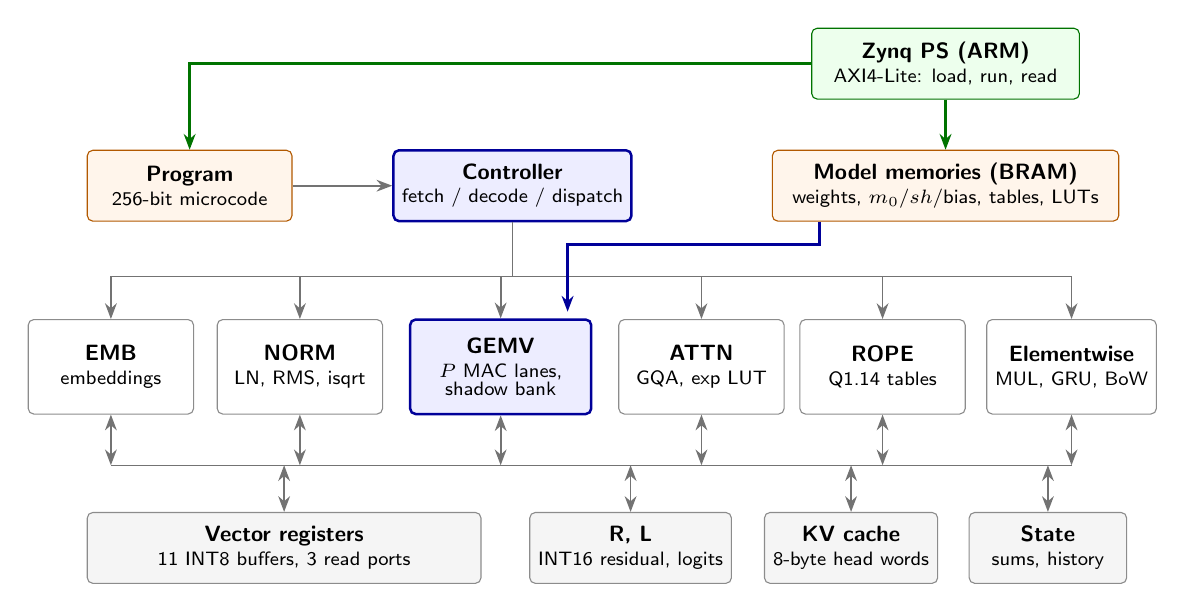
\begin{tikzpicture}[x=1cm,y=1cm, font=\sffamily\footnotesize,
  box/.style={draw=black!45, rounded corners=2pt, fill=white, align=center, minimum height=9mm, inner sep=3pt},
  acc/.style={box, draw=blue!60!black, fill=blue!7, line width=0.9pt},
  mem/.style={box, fill=black!4},
  ext/.style={box, draw=orange!70!black, fill=orange!8},
  ps/.style={box, draw=green!45!black, fill=green!7},
  flow/.style={-{Stealth[length=2mm]}, draw=black!55, line width=0.6pt}]
  \node[ext, minimum width=26mm] (prog) at (0.8,0) {\textbf{Program}\\[-1pt]\scriptsize 256-bit microcode};
  \node[acc, minimum width=30mm] (ctl) at (4.9,0) {\textbf{Controller}\\[-1pt]\scriptsize fetch / decode / dispatch};
  \node[ext, minimum width=44mm] (rom) at (10.4,0) {\textbf{Model memories (BRAM)}\\[-1pt]\scriptsize weights, $m_0$/$sh$/bias, tables, LUTs};
  \node[ps, minimum width=34mm] (ps7) at (10.4,1.55) {\textbf{Zynq PS (ARM)}\\[-1pt]\scriptsize AXI4-Lite: load, run, read};
  \draw[flow] (prog) -- (ctl);
  \draw[flow, draw=green!45!black, line width=0.9pt] (ps7) -- (rom);
  \draw[flow, draw=green!45!black, line width=0.9pt] (ps7.west) -| (prog.north);
  \foreach \n/\x/\t/\s in {emb/-0.2/EMB/{embeddings}, norm/2.2/NORM/{LN, RMS, isqrt},
                           attn/7.3/ATTN/{GQA, exp LUT}, rope/9.6/ROPE/{Q1.14 tables}, ew/12.0/Elementwise/{MUL, GRU, BoW}}
    {\node[box, minimum width=21mm, minimum height=12mm] (\n) at (\x,-2.3) {\textbf{\t}\\[-1pt]\scriptsize \s};}
  \node[acc, minimum width=23mm, minimum height=12mm] (gemv) at (4.75,-2.3) {\textbf{GEMV}\\[-1pt]\scriptsize $P$ MAC lanes,\\[-3pt]\scriptsize shadow bank};
  \draw[draw=black!55] (ctl.south) -- (4.9,-1.15);
  \draw[draw=black!55] (-0.2,-1.15) -- (12.0,-1.15);
  \foreach \n in {emb,norm,gemv,attn,rope,ew} \draw[flow] (\n.north |- 0,-1.15) -- (\n.north);
  \draw[flow, draw=blue!60!black, line width=1pt] (rom.south) ++(-1.6,0) |- (5.6,-0.75) -- (5.6,-1.6);
  \draw[draw=black!55] (-0.2,-3.55) -- (12.0,-3.55);
  \foreach \n in {emb,norm,gemv,attn,rope,ew} \draw[flow, {Stealth[length=2mm]}-{Stealth[length=2mm]}] (\n.south) -- (\n.south |- 0,-3.55);
  \node[mem, minimum width=50mm] (vrf) at (2.0,-4.6) {\textbf{Vector registers}\\[-1pt]\scriptsize 11 INT8 buffers, 3 read ports};
  \node[mem, minimum width=24mm] (rl) at (6.4,-4.6) {\textbf{R, L}\\[-1pt]\scriptsize INT16 residual, logits};
  \node[mem, minimum width=22mm] (kv) at (9.2,-4.6) {\textbf{KV cache}\\[-1pt]\scriptsize 8-byte head words};
  \node[mem, minimum width=20mm] (st) at (11.7,-4.6) {\textbf{State}\\[-1pt]\scriptsize sums, history};
  \foreach \m in {vrf,rl,kv,st} \draw[flow, {Stealth[length=2mm]}-{Stealth[length=2mm]}] (\m.north |- 0,-3.55) -- (\m.north);
\end{tikzpicture}
}
\caption{The microcoded engine. A controller fetches 256-bit instructions and dispatches them to one of seven units;
all model-specific content lives in memories that the Zynq PS loads at run time.}
\label{fig:engine}
\end{figure}

\textbf{Instruction set.} Table~\ref{tab:isa} lists the fifteen operations. A 256-bit instruction carries an opcode,
destination and two source buffers, a mode, four 16-bit sizes, two memory base addresses and two constants
($m_0$/$sh$, the normalization constants $K$ and $E$, or the softmax constant $C$ and shift $F$). The compiler emits the
program of a model (2 to 74 instructions) and its memory images; the controller executes the program once per token.

\begin{table}[t]
\centering\footnotesize
\caption{Engine operations.}
\label{tab:isa}
\setlength{\tabcolsep}{3pt}
\resizebox{\columnwidth}{!}{%
\begin{tabular}{@{}ll@{}}
\toprule
Operation & Semantics \\ \midrule
\code{EMB16}/\code{EMB8}/\code{EMBWIN} & embedding (+ position) / window of $k$ embeddings \\
\code{TABLOGIT}, \code{HRESET} & bigram logits; $h\leftarrow h_0$ at $t=0$ \\
\code{NORM} & LN/RMS over segments, INT16 or INT8 in/out \\
\code{GEMV} & $W[x;x']+b$; INT8 out, residual add, table, logits \\
\code{ROPE}, \code{KVSTORE}, \code{ATTN} & rotation; cache write; GQA softmax-average \\
\code{MUL}, \code{GRUUPD}, \code{COPY}, \code{REQ}, \code{BOW} & element-wise operations \\ \bottomrule
\end{tabular}}
\end{table}

\textbf{Units.} The GEMV unit is output-stationary with $P$ MAC lanes ($P=8$ unless stated): it streams one
$P$-byte weight word per cycle, accumulates $P$ outputs in INT32, and hands them to a shadow bank so that the serial
requantizer of block $b$ overlaps the accumulation of block $b+1$. A layer of $n_\mathrm{in}\times n_\mathrm{out}$ takes
$n_\mathrm{in}\lceil n_\mathrm{out}/P\rceil$ cycles; the input may be the concatenation of two buffers ($[x_t;h_{t-1}]$).
The NORM unit makes one pass, normalizes $Q$, takes a 28-cycle integer square root and one division. The attention unit has
8 lanes (the head size): a KV-cache word holds one head at one position, so a score and a weighted-value accumulation take
one cycle per cached position; a head costs $2(t+1)$ cycles plus one reciprocal. Divisions use a restoring divider that
starts at bit $Q_B$ when the quotient is known to be $<2^{Q_B}$ (41 instead of 64 cycles for normalization, 18 instead
of 34 for the softmax reciprocal). Element-wise units read up to three INT8 vectors per cycle.

\textbf{Cycle model.} Because every unit is a fixed state machine, the cycles of the token at position $t$ follow
from the microcode in closed form:
\begin{equation}
\begin{aligned}
C(t) ={}& 3 + 2N_\mathrm{instr} + \textstyle\sum_\mathrm{NORM} S\,(2n + 73) + C_\mathrm{other}\\
&+ \textstyle\sum_\mathrm{GEMV}\big[n_\mathrm{in} + (B-1)\max(n_\mathrm{in},P{+}2) + P + 5\big]\\
&+ \textstyle\sum_\mathrm{ATTN} H\,\big(2(t+1) + 30\big),
\end{aligned}
\label{eq:cycles}
\end{equation}
with $B=\lceil n_\mathrm{out}/P\rceil$ blocks per layer, $S$ normalization segments of length $n$, $H$ heads, and small
linear terms for the remaining operations ($C_\mathrm{other}$: embeddings $N{+}2$, RoPE $2+3d_h/2$ per head, element-wise
$n$ or $n{+}3$). Eq.~\eqref{eq:cycles} reproduces the simulated cycles of every model at every position exactly
(\zooPerfPairs{} (run, position) pairs, maximum deviation \zooPerfMaxErr{} cycles), so the hardware cost of an
architecture can be read off its program without simulation or synthesis.

\textbf{Storage.} Eleven INT8 vector buffers (P-byte words, byte-enable writes, three asynchronous read ports), the INT16
residual and logit memories, the KV cache, the running sums of the bag-of-words model and the token history are on chip.
Weights, requantization parameters, tables and activation tables are block RAMs.

\textbf{One bitstream.} With \code{LOADABLE=1} the model memories are RAMs written through a load port; an AXI4-Lite wrapper
exposes the load port, per-step control, a logit window, a hardware argmax and a cycle counter to the ARM cores of the
Zynq. The \emph{universal} configuration is sized for the maximum over all models ($V=512$, $T=256$, five layers); a
Python driver loads any model in milliseconds to seconds and runs it without re-synthesis. With \code{SPECIALIZE=1} the
units a model does not use are removed, which we use to attribute resources to architectural features.


% ===========================================================================
\section{Verification}\label{sec:verif}
% ===========================================================================
Every claim about the hardware rests on bit-exact equality with the integer reference. Table~\ref{tab:verif} summarizes
the evidence.

\begin{table}[t]
\centering\footnotesize
\caption{Verification evidence (all simulations with assertions on address ranges, INT32 accumulator overflow and the
divider's precondition).}
\label{tab:verif}
\setlength{\tabcolsep}{3pt}
\begin{tabular}{@{}p{0.43\columnwidth}p{0.5\columnwidth}@{}}
\toprule
Check & Result \\ \midrule
Every trained model, test set, all logits & \zooVerifRuns{} checkpoints, \zooVerifiedLogits{} logits, 0 mismatches \\
Same, specialized engine and load port & 0 mismatches \\
One-bitstream engine via AXI (10 models) & 0 mismatches; 200-token story identical \\
Randomized differential tests & \zooFuzzCases{} random architectures/sizes/weights, \zooFuzzLogits{} logits, 0 mismatches \\
4-state simulation (Icarus), X on outputs & 0 unknown logits \\
Divider, exhaustive ($W{=}12$) + random & \zooArithCases{} cases, 0 errors \\
Independent C implementation of the ISA & bit-exact on all models \\
On-board (PYNQ-Z2), all models & \zooBoardVerif{} \\ \bottomrule
\end{tabular}
\end{table}

The simulations use Verilator 5.052; the randomized tests draw an architecture, vocabulary (27--512), context (8--64),
depth (1--3) and width at random, fill the weights with values of random scale, calibrate on random tokens, and compare
every logit of random token sequences. The divider's skip-ahead is proven by exhaustive simulation of every valid input
at $W=12$ and by the property $q\,b\le a<(q+1)\,b$ on random 64-bit cases; the softmax reciprocal is checked for every
denominator in $[2^{15},2^{24})$. A third implementation, a C instruction-set simulator of the microcode, matches as well
and serves as the CPU baseline.


% ===========================================================================
\section{Results}\label{sec:results}
% ===========================================================================
% Results -- narrative written from the generated data (paper/data/), see sw/zoo/paper_data.py.
\subsection{Quality and cost of the nine architectures}\label{sec:res-family}
\begin{table}[t]
\centering\footnotesize
\caption{Names, 50k-parameter budget: test loss (nats/token, mean $\pm$ s.d. over seeds), INT8 loss increase, engine
cycles per token and resources of the specialized engine (Yosys, XC7Z020).}
\label{tab:family-res}
\setlength{\tabcolsep}{2.5pt}
\begin{tabular}{@{}lrrrrrr@{}}
\toprule
Model & Params & Test loss & $\Delta_\mathrm{INT8}$ & Cycles & LUT & DSP \\ \midrule
\tabinput{data/tab_family.tex}
\bottomrule
\end{tabular}
\end{table}

\subsection{What each idea costs: the feature ladder}\label{sec:res-ladder}
\subsection{Context length: when does attention pay off?}\label{sec:res-context}
\subsection{Scale}\label{sec:res-scale}
\subsection{Where the INT8 error comes from}\label{sec:quant}
\subsection{Engine design space and the one-bitstream engine}\label{sec:res-dse}
\subsection{On-board measurements}\label{sec:res-board}


% ===========================================================================
\section{Discussion and limitations}\label{sec:discussion}
% ===========================================================================
% Discussion: the result-dependent paragraphs are written from paper/data once the campaigns are complete.
% generated / written once the campaigns are complete


\textbf{Limitations.} The models are small (12k--260k parameters) and the conclusions about architectures are drawn at
this scale; Narang et al.\ \cite{narang2021transformer} show that architectural conclusions do not always transfer across
scales, and outlier behaviour changes with scale \cite{dettmers2022llmint8}. On TinyStories every model is trained once
(one seed, one learning rate) for compute reasons. All weights and the KV cache are on chip, which bounds the model size on
the XC7Z020 at roughly the size of stories260K; larger models need weights streamed from DDR, which changes the
performance model from compute-bound to bandwidth-bound. The attention unit assumes a head size of 8. Resource numbers
for every model come from open-source synthesis (Yosys) without timing; post-route utilization, timing and power for the
one-bitstream engine come from Vivado (\S\ref{sec:res-board}). Energy is measured at the board input with a USB meter,
which includes the PS and the DDR; we therefore report dynamic power above idle.

\textbf{Reproducibility.} The repository contains the training campaigns (seeds, learning-rate sweeps, logs), the
compiler, the integer reference, the generated memories and golden vectors of every model, the RTL and testbenches, the
Vivado scripts for the overlay and the out-of-context sweep, the PYNQ driver and measurement scripts, and the scripts that
generate every table and figure of this paper from the raw results. A continuous-integration job re-runs the bit-exact
regression on every commit.


% ===========================================================================
\section{Conclusion}
% ===========================================================================
% written once the results are final


\bibliographystyle{IEEEtran}
\bibliography{refs}
\end{document}
